\chapter{Fundamentação Teórica}
\label{c.fundamentacaoteorica}

A utilização e implementação de bibliotecas externas, assim como a comunicação entre diferentes linguagens tem aproximado a interação que ocorre nas linguagens de programação com a interação de linguagens naturais.

A forma de transmissão dos dados caracteriza uma arquitetura de informação.  \citeauthoronline{hollan} (\citeyear{hollan}) dizem que:

\begin{quotation}
``Processos cognitivos envolvem trajetórias de informações (de transmissão e transformação), de modo que os padrões destas trajetórias de informação, se estáveis, refletem uma arquitetura cognitiva subjacente. Uma vez que a organização social - mais a estrutura adicionada ao contexto da atividade - determina em grande parte o modo como a informação flui através de um grupo, a organização social em si pode ser vista como uma forma de arquitetura cognitiva.''
\end{quotation}

Dessa forma o desenvolvimento modular não se dá somente por convenção e facilidade de implementação, como também cumpre um papel de definição organizacional entre várias bibliotecas e estruturas de dados.

\section{Audio Fingerprint}
\label{s.audiofingerprint}

Um audio fingerprint é definido por  \citeauthoronline{canoetal05} (\citeyear{canoetal05}, tradução nossa) como uma assinatura única de uma música, contendo um sumário de suas características. \citeauthoronline{canoetal05} (\citeyear{canoetal05}, tradução nossa) definem que um sistema ideal de fingerprint deve identificar um item, independentemente do nível de compressão, distorção ou interferência no canal de transmissão . E definem também que esse sistema pode ser separado em dois processos fundamentais: extração do fingerprint, e o algoritmo de comparação.

O processo completo de extração de dados pode ser divido nos tópicos:

\begin{alineas}

\item Pré-processamento
\item Enquadramento
\item Transformada
\item Extração de características
\item Pós-processamento
\item Modelagem do fingerprint
\item Busca e acesso à base de dados
\item Teste de acerto

\end{alineas}

\begin{figure}[h]
\caption{\small Diagrama de identificação de áudio.}
\centering
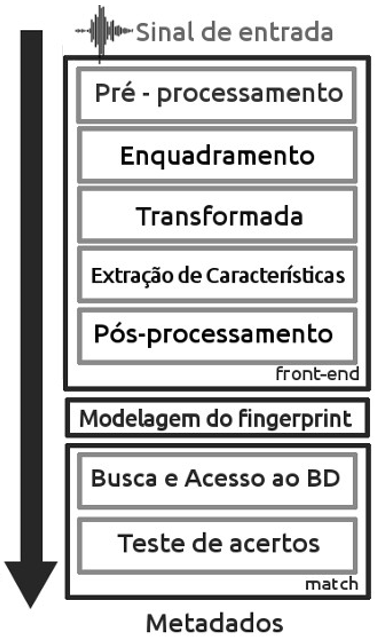
\includegraphics[scale=0.50]{figs/arquitetura.png}
\label{f.diagrama}
\legend{\small Fonte: Elaborada pelo autor.}
\end{figure}

\subsection{Pré-processamento}
\label{ss.preprocessamento}

Para que o processamento e que a extração de características tome o menor tempo computacional possível, o sinal passará por um filtro que removerá dados que não interessam à extração de características, segundo \citeauthoronline{canoetal05} (\citeyear{canoetal05}, tradução nossa): convertendo para o formato de 16 bits PCM\footnote{Pulse-code modulation: método usado para representação digital de sinais analógicos.}, agrupando através da média os canais esquerdo e direito em uma taxa de amostragem variando de 5 a 44,1 kHz.

\subsection{Enquadramento}
\label{ss.enquadramento}

O enquadramento adapta a amostragem para o que será utilizado. \citeauthoronline{canoetal05} (\citeyear{canoetal05}) definem o enquadramento dizendo que:

\begin{quotation}
``Um pressuposto fundamental na medição das características é que o sinal pode ser considerado como estacionário em um intervalo de alguns milissegundos. Portanto, o sinal é dividido em quadros de dimensão comparável à velocidade de variação dos eventos acústicos subjacentes. O número de quadros computados por segundo é chamado de taxa de quadros. Uma função de janela é aplicada a cada bloco para minimizar as descontinuidades entre o início e o fim. Uma justaposição deve ser aplicada para garantir robustez para o deslocamento (isto é, quando os dados de entrada não forem perfeitamente alinhados). E é necessário equilibrar os valores acima entre a taxa de variação no espectro e complexidade do sistema''
\end{quotation}

\subsection{Transformada}
\label{ss.transformada}

A complexidade do sistema define como será tratado o enquadramento, para que o algoritmo de reconhecimento possa realizar uma melhor classificação dentro das características desejadas.

Os sinais sonoros que observamos são captados em função do tempo, mas ao aplicar transformadas que convertam esses sinais em função da frequência é possível observar particularidades que não podiam ser observadas anteriormente, assim como também é possível fazer um reconhecimento de padrões desses sinais em função da frequência. A transformada de Karhunen-Loève é uma transformada que consegue comprimir de maneira ótima os dados referentes ao sinal  (\citeauthoronline{raok} , \citeyear{raok}), mas depende da função de entrada, tornando o cálculo computacional demasiadamente intensivo. \citeauthoronline{canoetal05} (\citeyear{canoetal05}) também cita a decomposição em valores singulares como uma compressão ótima porém impraticável. Outras transformadas são citadas que podem ser utilizadas para extrair características:

\begin{alineas}

\item Tranformada rápida de Fourier
\item Transformada de Walsh-Hadamard
\item \emph{Modulated Complex Lapped Transform (MCLT)}
\item Transformada Wavelet

\end{alineas}


\subsection{Extração de Características}
\label{ss.extracaocaracteristicas}

Os dados obtidos pela transformada serão novamente transformados de modo que aumente a sua invariânica a distorções do som, como aumento do pitch ou mudança do tempo. Características que fazem parte do objetivo são levadas em conta nessa fase, como frequências relevantes (no caso de extração de voz ou reconhecimento de instrumentos), harmonicidade e ruído (no caso de classificação musical).

\subsection{Pós-processamento}
\label{ss.posprocessamento}

Para complementar os dados absolutos, as variações temporais podem ser adicionadas ao sinal processado, através das derivativas de primeira e segunda ordem.

Os metódos da primeira fase onde o sinal é pré-processado até aqui são agrupados e podem ser classificados como o front-end da obtenção do fingerprint.

\subsection{Modelagem do Fingerprint}
\label{ss.modelagemfingerprint}

A modelagem do fingerprint usualmente recebe uma sequência de vetores de características calculadas quadro a quadro \citeauthoronline{canoetal05} (\citeyear{canoetal05}, tradução nossa). As características que serão usadas para montar o modelo do fingerprint influenciam a forma como o algoritmo irá tratar futuramente a busca dessas características para comparação. Os processos mais simplificados como o de softwares como o \emph{Music-brainz} traduzem as características para um hash de identificação, outros mais complexos armazenam o modelo em um formato de vetor ou matriz bidimensional.

\subsection{Busca e acesso ao BD}
\label{ss.buscabd}

A Busca depende diretamente do modelo definido e do problema a ser resolvido, pois nesse passo é preciso classificar o peso de cada característica extraída e a métrica utilizada para encontrar a distância entre cada fingerprint. O Banco de dados armazena os fingerprints já identificados e pode criar indíces de busca para campos de maior relevância, para diminuir o custo computacional da comparação.

\subsection{Teste de Acertos}
\label{ss.testeacertos}

Para identificação do fingerprint, ele passa por um teste de cálculo da probabilidade de acerto, onde é verificado se pertence ou não ao banco de dados atual, podendo ser classificado como pertencente ou não. Deve-se definir um limite de aceitação para classificar também um dado falso positivo (no caso de um banco de dados muito grande) ou um falso negativo (no caso de dados insuficientes).


\section{Chromaprint}
\label{s.chromaprint}

Segundo \citeauthoronline{chromaprint} (\citeyear{chromaprint}, tradução nossa) a música popular é frequentemente baseada em uma estrutura simples que pode alternar entre versos e um refrão ou acorde repetido. Uma estratégia razoável para selecionar uma representação musical nestes casos mais simples envolve a localização e identificação destas seções que se repetem.

\subsection{PCP - \emph{Pitch Class Profile} }
\label{ss.pcp}

\citeauthoronline{shepard} (\citeyear{shepard}, tradução nossa) diz que uma nota tocada nos remete a várias propriedades de percepção. Uma é o pitch, que é a qualidade do som determinada pela taxa de vibrações que produz; o grau agudo ou grave de um tom. Outra é a similaridade entre os intervalos de pitch, que também são chamadas de  ``cores'' da nota, essa propriedade pode ser classificada como a escala de notas e denominada o \emph{chroma} da nota, ou \emph{pitch class profile}.
\begin{figure}[h]
\caption{\small Illustração da hélice de Shepard sobre percepção do \emph{pitch}. O eixo vertical representa a altura do tom e a dimensão angular representa o \emph{chroma}}
\centering
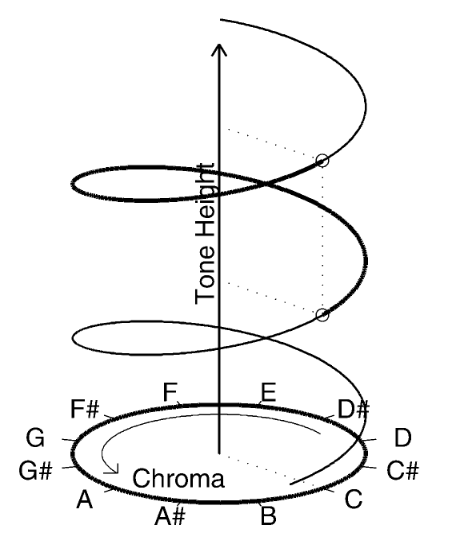
\includegraphics[scale=0.8]{figs/chromaperception.png}
\label{f.chromaperception}
\legend{\small Fonte:  \cite{chromaprint}.}
\end{figure}


\subsection{\emph{Chroma} musical e a música ocidental }
\label{ss.westmusic}

Na teorica musical ocidental o sistema de tons divide cada oitava em doze partes iguais, classificando a frequência de 440Hz como um lá (A), e progredindo a escala logaritmamente a partir dessa frequência até repetir novamente a sensação cromática do lá, alcançada na frequência de 880Hz, esse intervalo entre as duas notas é denominado uma oitava, e dividido em 12 partes iguais, essa divisão é chamada de escala cromática.

\begin{figure}[h]
\caption{\small Representação da escala cromática iniciando em um Dó (C).}
\centering
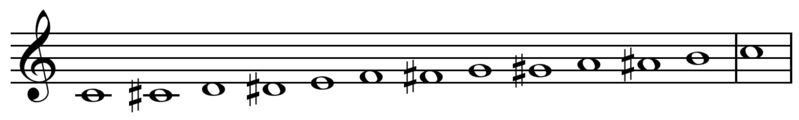
\includegraphics[scale=0.6]{figs/escalacromatica.png}
\label{f.chromaticn}
\legend{\small Fonte:  Elaborada pelo autor.}
\end{figure}

Devido a repetição de frequência e similaridade de notas, podemos representar as notas de uma música em um vetor de 12 posições, um para cada classe de \emph{pitch}. Essa representação nos permite extrair características musicais através de uma DFT\footnote{Discrete Fourier transform - Transformação discreta de Fourier}:

\begin{figure}[h]
\caption{\small Representação colorida de \emph{chroma features}.}
\centering
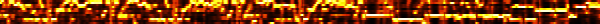
\includegraphics[scale=0.6]{figs/chr.png}
\label{f.chromaticn}
\legend{\small Fonte:  \cite{chromaworks}.}
\end{figure}

\subsection{Comparação de fingerprint por filtro visual.}
\label{ss.visual}

\cite{pasteldeflango} definem um algoritmo de comparação de dois \emph{audio fingerprints} com base em um filtro visual de soma de características. Existem dezesseis tipos de filtros aplicados a uma janela de tamanho de 16x12 pixels, cada filtro é aplicado para capturar diferentes intensidades musicais.

\begin{figure}[h]
\caption{\small Formas de arranjo dos filtros visuais.}
\centering

\includegraphics[scale=1]{figs/filters.png}
\label{f.chromaticn}
\legend{\small Fonte:  \cite{chromaworks}.}
\end{figure}

Segundo \citeauthoronline{chromaworks} (\citeyear{chromaworks}, tradução nossa) para cada filtro é calculada a diferença da soma das áreas brancas com a soma das áreas pretas. Cada filtro tem três coeficientes associados a ele, que guiam como classificar o resultado de 0 a 3. Esse filtros e coeficientes foram selecionados por um algoritmo de aprendizado de máquina, treinado durante o desenvolvimento da biblioteca.

\begin{figure}[h]
\caption{\small Diferença bit a bit de duas versões da música, uma sem compressão e a outra comprimida em MP3.}
\centering
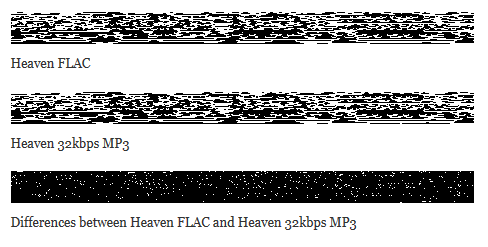
\includegraphics[scale=1]{figs/heavendifferences.png}
\label{f.chromaticn}
\legend{\small Fonte:  \cite{chromaworks}.}
\end{figure}

O resultado dos 16 filtros produzem um inteiro que pode ser codificado em 2 bits, combinando os resultados temos um inteiro de 32 bits, se aplicarmos estes filtros para cada janela dos \emph{chroma features} obtemos um \emph{audio fingerprint} completo.

Com base nesse fingerprint a busca por proximidade em um banco de dados pode ser otimizada para encontrar uma música que esteja mais próxima da música procurada, mesmo que em versões diferentes.

\begin{figure}[h]
\caption{\small Diferença entre as versões originais e instrumentais de duas músicas.}
\centering
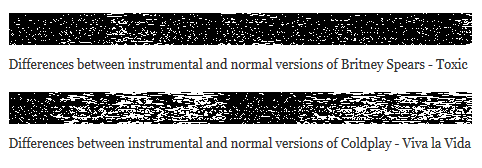
\includegraphics[scale=1]{figs/instrumental.png}
\label{f.chromaticn}
\legend{\small Fonte:  \cite{chromaworks}.}
\end{figure}
